% SECTION ====================================================================================
\vspace{-4pt}
\begin{sectionbox}
\section{Hashing}
% ============================================================================================
\subsection{Motivation und Idee}\smallskip
Key/Value-Paare effizient abspeichern und finden z.B. für Implementation eines Dicts oder einer Datenbank.\par\smallskip

\begin{center}
    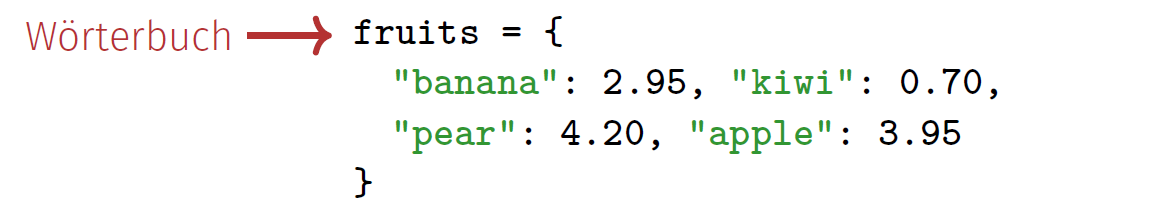
\includegraphics[width = 0.8\columnwidth]{../img/BspPreHashing.png}
\end{center}\smallskip

\textbf{Idee}\par
Direkter Zugriff (Array)\par\smallskip
\begin{greenbox}
\textbf{Probleme}\par
\begin{enumerate}
    \item \textbf{Schlüssel müssen nichtnegative ganze Zahlen sein}
    \item \textbf{Grosser Schlüsselbereich $\rightarrow$ grosses Array}
\end{enumerate}
\end{greenbox}
\end{sectionbox}
\vspace{-4pt}
\begin{sectionbox}
\subsection{Pre-Hashing: Lösung des ersten Problems}\smallskip
Prehashing: Bilde Schlüssel ab auf positive Ganzzahlen mit einer Funktion $ph: \mathcal{K} \rightarrow \mathbb{N}$\par\smallskip
\textbf{Pre-Hashing: Beispiel String}\par
Zuordnung Name $s=s_{1} s_{2} \ldots s_{l_{s}}$ zu Schlüssel\par\smallskip
\begin{center}
    $\operatorname{ph}(s)=\left(\sum_{i=0}^{l_{s}-1} s_{l_{s}-i} \cdot b^{i}\right) \bmod 2^{w}$
\end{center}\par\smallskip
$b$ so, dass verschiedene Namen möglichst verschiedene Schlüssel erhalten.
$w$ Wortgrösse des Systems (z.B. 32 oder 64).\par\smallskip
\begin{lstlisting}[language=C++]
#include <string>
unsigned prehash(std::string s) {
    unsigned b = B;
    unsigned h = 0;
    
    for (unsigned i = 0; i < s.size(); ++i){
        h = h * b + s[i];
    }
    return h;
}
\end{lstlisting}\vspace{-6px}
\end{sectionbox}
\vspace{-4pt}
\begin{sectionbox}
\subsection{Hashing: Lösung des zweiten Problems}\smallskip
Reduziere des Schlüsseluniversum: Abbildung (Hash-Funktion) $h: \mathcal{K} \rightarrow\{0, \ldots, m-1\}(m \approx n=\text { Anzahl Einträge in der Tabelle })$\par\vspace{7px}

\subsubsection{Nomenklatur}\par\smallskip
\textbf{Hashfunktion} $h$: Abbildung aus der Menge der Schlüssel $\mathcal{K}$ auf die Indexmenge $\{0,1, \ldots, m-1\}$ eines Arrays (\textbf{Hashtabelle})\par
Meist $|\mathcal{K}| \gg m$, Es gibt also $k_{1}, k_{2} \in \mathcal{K}$ mit $h\left(k_{1}\right)=h\left(k_{2}\right)$ (\textbf{Kollision}). Eine Hashfunktion sollte die Menge der Schlüssel möglichst gleichmässig auf die Positionen der Hashtabelle verteilen.\par\vspace{7px}

\subsubsection{Gebräuchliche Hashfunktion: Divisionsmethode}\par\smallskip
\begin{center}
    $h(k)=k \bmod m$
\end{center}
Ideal: $m$ Primzahl, nicht zu nahe bei Potenzen von 2 oder 10\par
Aber oft: $m=2^{k}-1(k \in \mathbb{N})$
\end{sectionbox}
\vspace{-4pt}
\begin{sectionbox}
\subsection{Konzept 1: Hashing mit Verkettung}\par\smallskip
Direkte Verkettung der Überläufer.\par
$\rightarrow$ Resultuiert im worst case in $\Theta(n^{2})$ pro Operation\par\smallskip

\textit{Beispiel}\par
\begin{center}
    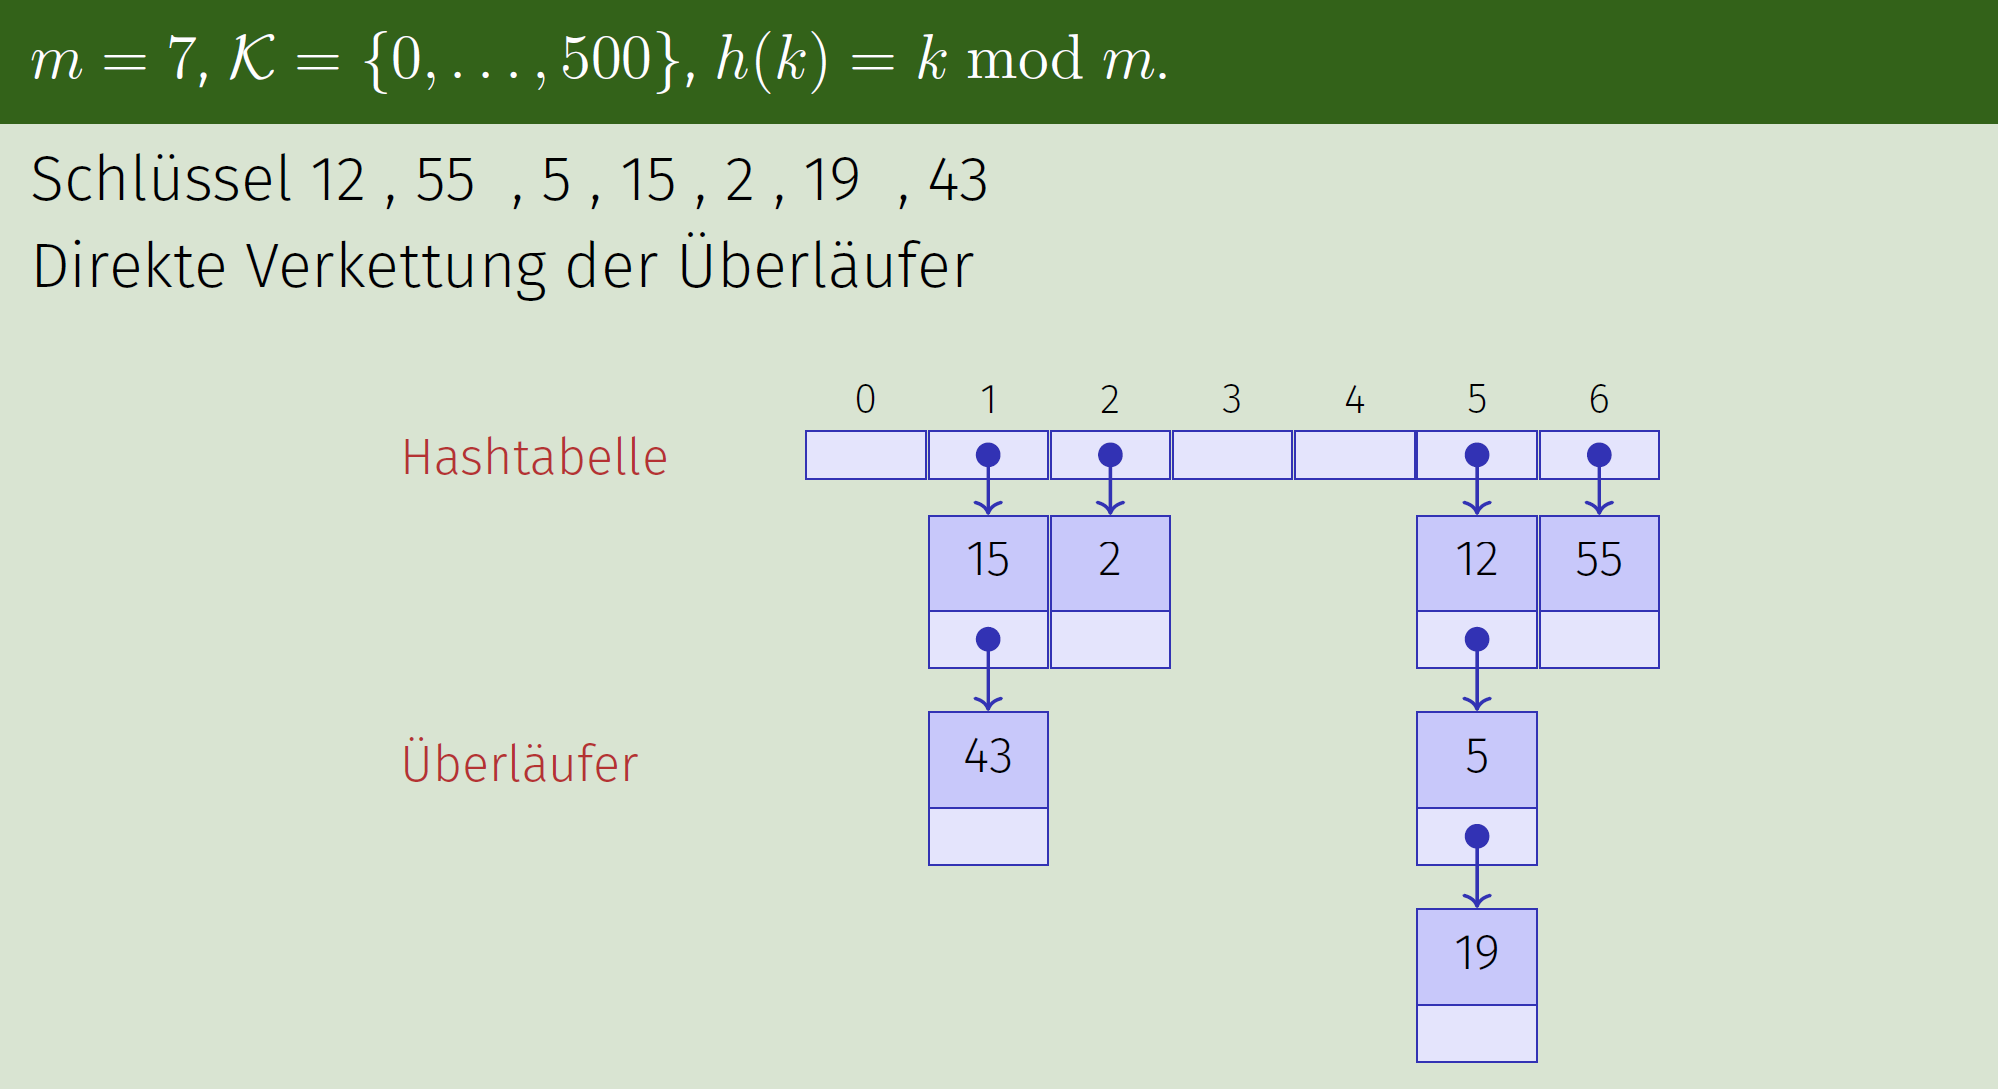
\includegraphics[width = \columnwidth]{../img/hashVerkettung.png}
\end{center}\smallskip

\textbf{Einfaches gleichmässiges Hashing}\par
Starke Annahmen: Jeder beliebige Schlüssel wird mit gleicher Wahrscheinlichkeit (\textbf{Uniformität}) und unabhängig von den anderen Schlüsseln (\textbf{Unabhängigkeit}) auf einen der $m$ verfügbaren Slots abgebildet.\par\smallskip
Unter dieser Annahme ergibt sich die \textbf{erwartete Länge}:\par $\mathbb{E}(\text { Länge Kette } j)=\frac{n}{m}=\alpha$, $\alpha$ heisst der \textbf{Belegungsfaktor} oder \textbf{Füllgrad}.\par\smallskip
Daraus ergibt sich (bei einfachem gleichmässigem Hashing) eine \textbf{erwartete Laufzeit (amortisiert)} von $\mathcal{O}(1)$ für Suchen, Einfügen, Löschen.\par\smallskip
\textbf{Vor- und Nachteile der Verkettung}\par
\begin{itemize}
    \item Belegungsfaktoren $\alpha > 1$ möglich; Entfernen von Schlüsseln einfach
    \item Speicherverbrauch der Verkettung
\end{itemize}\smallskip

\end{sectionbox}
\vspace{-4pt}
\begin{sectionbox}
\subsection{Konzept 2: Hashing mit offener Addressierung}\par\smallskip
\begin{itemize}
    \item Speichere die Überläufer direkt in der Hashtabelle mit einer \textbf{Sondierungsfunktion $s(k,j)$}
    \item Tabellenposition des Schlüssels entlang der \textbf{Sondierungsfolge $S(k)$}
\end{itemize}\par\smallskip
Technisches Detail zu \textbf{delete(k)}: Suche $k$ in der Tabelle gemäss $S(k)$. Ersetze $k$ durch den \textbf{speziellen Schlüssel removed}.\par\vspace{7px}
\end{sectionbox}
\vspace{-4pt}
\begin{sectionbox}
\subsubsection{Lineares Sondieren}\par\smallskip
\begin{center}
    $s(k, j)=h(k)+j \Rightarrow$ \par $S(k)=(h(k), h(k)+1, \ldots, h(k)+m-1) \bmod m$
\end{center}\par\smallskip
\textbf{Problem $\rightarrow$ Primäre Häufung}:\par Ähnliche Hashaddressen haben ähnliche Sondierungsfolgen $\rightarrow$ lange zusammenhängende belegte Bereiche.\par\smallskip
\textit{Beispiel}\par
\begin{center}
    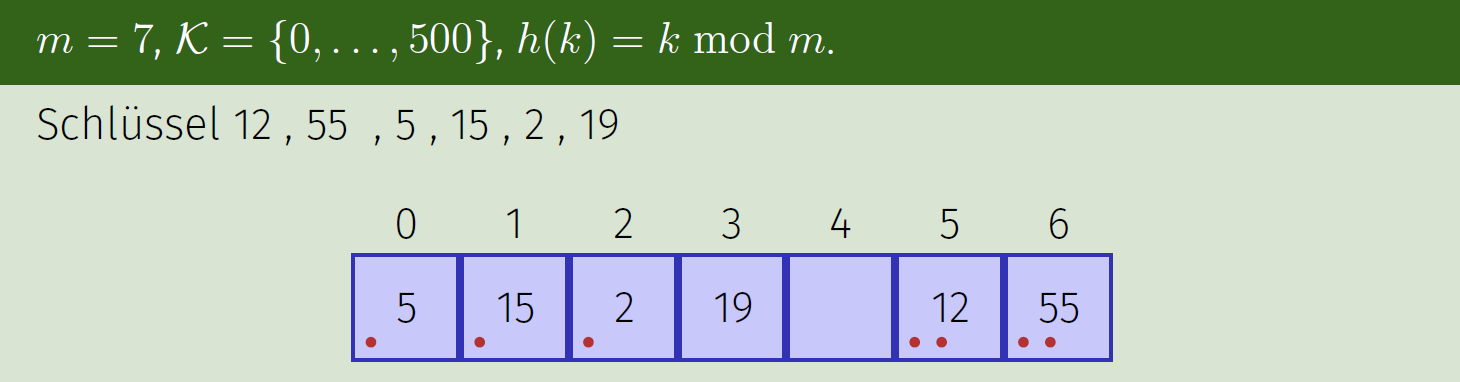
\includegraphics[width = 0.9\columnwidth]{../img/BspLinSond.png}
\end{center}
\end{sectionbox}
\vspace{-4pt}
\begin{sectionbox}
\subsubsection{Quadratisches Sondieren}\par\smallskip
\begin{center}
    $s(k, j)=h(k)+\lceil j / 2\rceil^{2}(-1)^{j+1}$
    $S(k)=(h(k), h(k)+1, h(k)-1, h(k)+4, h(k)-4, \ldots) \bmod m$
\end{center}\par\smallskip
\textbf{Problem $\rightarrow$ Sekundäre Häufung}:\par Synonyme $k$ und $k^{\prime}\left(\operatorname{mit} h(k)=h\left(k^{\prime}\right)\right)$ durchlaufen dieselbe Sondierungsfolge.\par\smallskip
\textit{Beispiel}\par
\begin{center}
    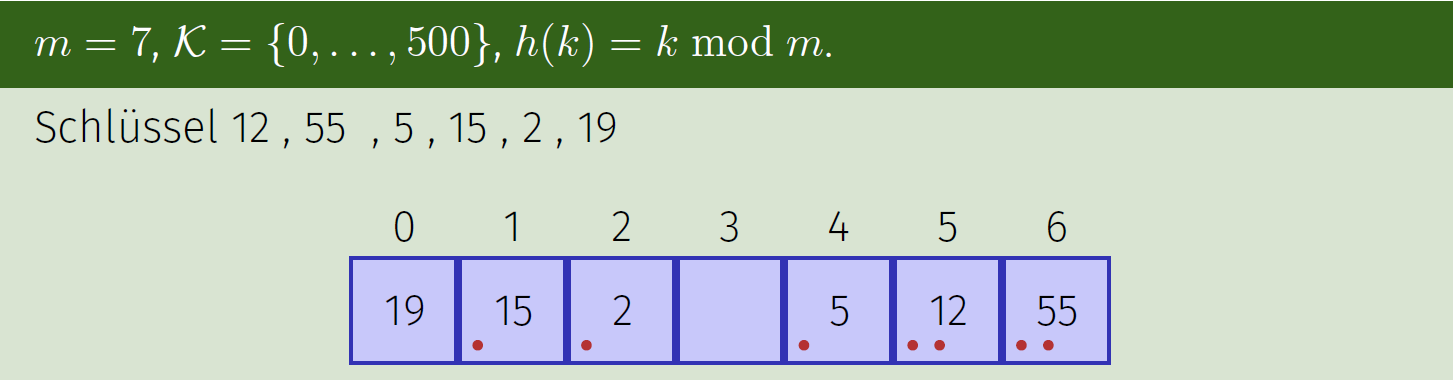
\includegraphics[width = 0.9\columnwidth]{../img/BspQuadSond.png}
\end{center}
\end{sectionbox}
\vspace{-4pt}
\begin{sectionbox}
\subsubsection{Double Hashing}\par\smallskip
Verwendung von zwei Hashfunktionen $h(k)$ und $h^{\prime}(k) \rightarrow$ Vermeidung primärer und sekundären Häufungen.
\begin{center}
    $s(k, j)=h(k)+j \cdot h^{\prime}(k)$\par
    $S(k)=(h(k), h(k)+h^{\prime}(k), h(k)+2 h^{\prime}(k)b, \ldots$ \par
    $, h(k)+(m-1) h^{\prime}(k)) \quad \bmod m$
\end{center}\par\smallskip

\textbf{Gleichmässiges Hashing}\par
Starke Annahme: Die Sondierungssequenz $S(k)$ eines Schlüssels $k$ ist mit gleicher Wahrscheinlichkeit eine der $m !$ vielen Permutationssequenzen von $\{0,1, \ldots, m-1\}$.
$\rightarrow$ Füllgrad $\alpha=$ $\frac{n}{m}<1$, so hat die nächste Operation erwartete Laufzeitkosten von $\leq \frac{1}{1-\alpha}$\par\smallskip
\textit{Beispiel}\par
\begin{center}
    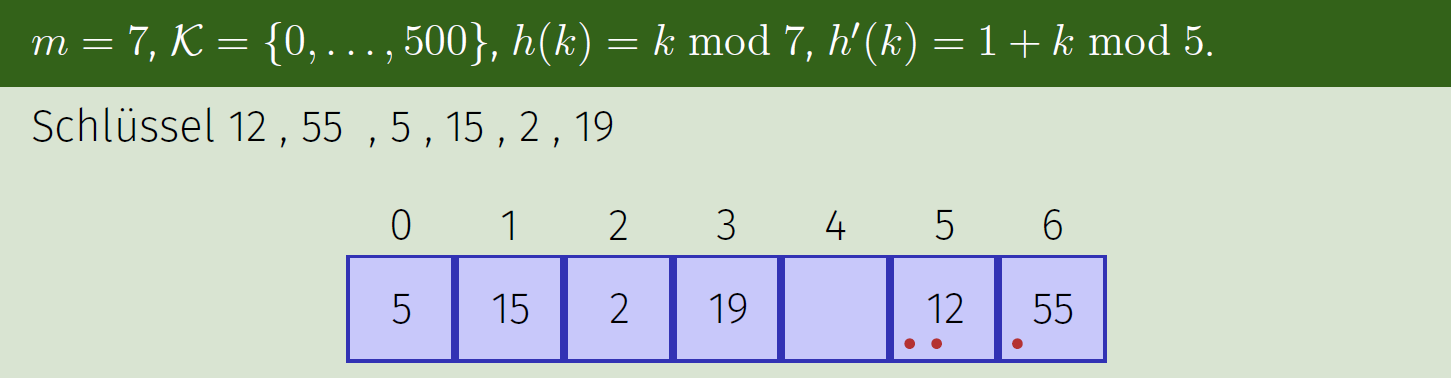
\includegraphics[width = 0.9\columnwidth]{../img/BespDoubHash.png}
\end{center}
\end{sectionbox}
\vspace{-4pt}
\begin{sectionbox}
\subsubsection{Beispiele}\par\smallskip
\begin{itemize}
    \item $h'(k) = \lceil \ln (k+1) \rceil \bmod q$: This function is not suitable as a second hash function, because for the key $k = 0$ we have $h'(0) = \lceil \ln (1) \rceil = 0$.
    \item $s(j,k) = k^j \bmod p$: This function is not suitable as a probing function, because for the keys $k = 0$ and $k = 1$, the function $s(j, k)$ has constant value of 0 and 1.
    \item $s(j,k) = ((k \cdot j) \bmod q) + 1$: This function is also not suitable as a probing function because its value is constant 1 if the key $k$ is a multiple of $q$.\par Moreover, for all other keys, the image of $s(j, k)$ is $\{1, . . . , q\}$, i.e., $p - q$ addresses of the hash table cannot be reached.
\end{itemize}

\end{sectionbox}